\documentclass[12pt]{report}

\usepackage{amsmath}
\usepackage[utf8]{inputenc}
\usepackage[norsk]{babel}
\usepackage{listings}
\usepackage{graphicx}
\usepackage{caption}
\usepackage{verbatim}
\usepackage{float}
\usepackage{pgfplots}
\restylefloat{table}

\title{TMM4850: Prosjektrapport}
\author{Christopher Tannum \\ Sindre Raknes \\ Audun 							Stensgaard \\ Tom Meland Pedersen \\ Tor-Håkon 							Bonsaksen}
\date{April 2015}



\begin{document}

\begin{titlepage}
    \begin{center}
        \vspace*{2.5cm}
        
        \Huge
        \textbf{TMM4850: Prosjektrapport}
        
        \vspace{0.5 cm}
        
        \large
        Gruppe E
        
        \vspace{2cm}
        
        
        \Large
        \textit{Christopher Tannum \\ Sindre Raknes \\ Audun 							Stensgaard \\ Tom Meland Pedersen \\ Tor-Håkon 							Bonsaksen}
        
    
    \end{center}
\end{titlepage}


\chapter*{
    \begin{center}
        Abstract
    \end{center}
}

Parallel programming is without a doubt something that any modern programmer needs in his/her toolbox. 
As the physical limits of a single processing unit is reached, parallel computers, both local and distributed are needed to continue to increase processing power. 
OpenMP and MPI are libraries that can be used to develop parallel programs with shared memory(OpenMP and MPI) and distributed systems(MPI).
Even though many serial algorithms can be made fully/partly parallel, the implementation can vary its efficiency.
It is therefor necessary for the programmer to take great care in choosing parallelization techniques for the problem.


\tableofcontents


\chapter{Introduksjon}
Denne rapporten vil gå i dybden og forklare i detalj de ulike aspektene ved oppgaven.
Først forklares oppgaven og de forskjellige elementene den består av. Deretter vil den overordnede arkitekturen bli gjennomgått etterfulgt av en gjennomgang av klient, server og enhet, som er kjerneelementene i prosjektet.
Eksempler på hva andre kan lage ved hjelp av APIet vil vises frem og til slutt vil det bli listet opp ting som kan jobbes videre med i fremtiden.

\section{Prosjektbeskrivelse}
Oppgaven gruppen kom frem til var å produsere et bibliotek / API som gjør det mulig og styre Dynamixel servoer[referanse] over ett nettverk. Produktet vi har laget vil hovedsaklig være et verktøy for andre utviklere men vi har laget noen demo applikasjoner for å vise frem hva man kan lage med biblioteket. Problemet med det som eksisterer fra før, er at det er proprietært og reduserer muligheten utviklere har når de skal lage programvare som benytter servoene.

\subsection{Dynamixel AX-12}
Dynamixel AX-12 er servoer med dedikerte mikrokontrollere som produseres av Robotis, et Sør-Koreansk selskap. De brukes av hobbyentusiaster og opplæringsinstitusjoner verden rundt til å modellere og simulere roboter, kjøretøyer og andre konfigurasjoner. De er ettertraktet fordi de er billige, robuste og svært fleksible. De er også lette å ta i bruk, mye på grunn av de dedikerte mikrokontrollene som styrer hver individuelle servo.

Elementært sett, har servoene tre input pinner, en for strøm, en for jording og den siste er en seriell datalinje. Hvis man skal ha flere servoer kobles de sammen i serie og de individuelle servoene styres ved at hver enkelt servo har sin unike ID. Servoene drives av en spenning på 9-12 volt.

\begin{figure}[h!]
	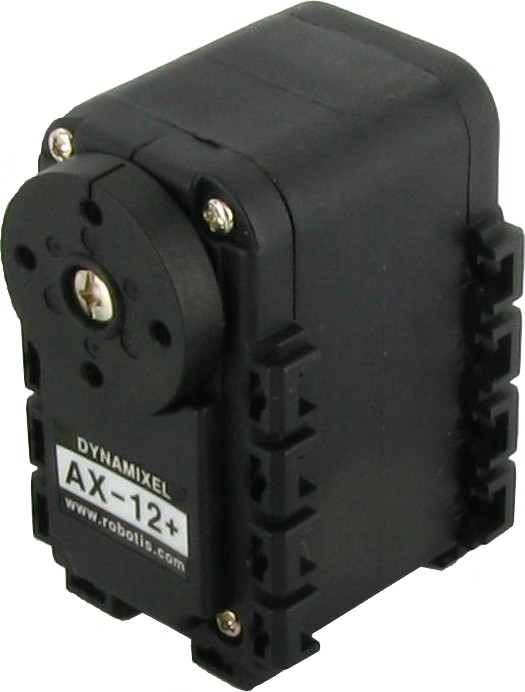
\includegraphics[scale=0.3]{servo_ax12-5}
	\centering
\end{figure}

Dataene som blir sendt gjennom data bussen blir sendt som heksadesimale pakker strukturert som [ref bilde]. På denne måten kan man sette konfigurasjoner som blant annet hastighet og posisjon. Vi kommer ikke til og gå i detalj på hvordan dette fungerer men mer informasjon kan finnes i Dynamixel AX-12 manualen [ref].

\subsection{Bruksområder}
Det som finnes av offisiell støtte for Dynamixel AX-12 servoene fra før er proprietært, og har ikke åpen kildekode. Dette gjør det vanskelig for utviklere og lage egen programvare, spesielt over nettverk. Programvaren vi utvikler vil åpne opp og gjøre det enklere for andre utviklere og lage spennende og sammfunnsnyttige applikasjoner. 

Løsningen vi tilbyr åpner for et stort antall utviklingsområder. I hovedsak så er det opplæringsinstitusjoner som vil kunne ha nytte av det vi lager. Studenter ved neste års Instrumentering og Styring over internett, har stor kreativ frihet til å enten bygge videre eller lage noe helt nytt. Eksempler på videre utvikling er:

\begin{itemize}
	\item Feste på et kamera og bruke det til å innhente informasjon.
	\item Kan utforske steder som er dårlig egnet for personer.
	\item Kan lage andre ting enn kjøretøy - Sluser, fjernstyrte servoapplikasjoner.
\end{itemize}

\clearpage

\chapter{Arkitektur}
Dette kapittelet beskriver arkitekturen og er ment å gi en overordnet oversikt over de forskjellige delene av prosjektet og hvordan de henger sammen. Mer detaljerte beskrivelser av de forskjellige delene kommer senere i rapporten.

\section{Server-Klient Arkitektur}
Arkitekturen som ble implementert er skildret ved en figur[ref] viser hvordan de forskjellige elementene i prosjektet henger sammen. Punkt 1 er selve enheten som består av en Raspberry pi[ref] som er koblet til servoene. Denne enheten kommuniserer med en ekstern server (2) gjennom sockets[ref]. Serveren (2) håndterer alt av forbindelser mellom brukere og enhetene. Når en enhet kobler seg til, vil den registrere seg med et navn, dette navnet kan så benyttes av brukere for og kommunisere med enheten. Del 3 av prosjektet er selve brukeren. Det kan være alt fra en applikasjon på telefon til styring med en dedikert kontroller. Applikasjonen pakker instruksjoner inn i et JSON objekt[ref] og sender det til serveren. Serveren sjekker at formatet er riktig strukturert og sender det videre til riktig enhet.

\section{Andre Mulige Arkitekturer}
Det var flere forskjellige typer arkitekturer som ble vurdert før utviklingen av prosjektet begynte. Arkitekturene ble sammenlignet ved positive og negative egenskaper med tanke på interesse av oppgaven, gjennomførbarhet og hva vi ønsket og oppnå. Til slutt satt vi igjen med en arkitektur som gruppen mente fungerte best til prosjektet.

\subsection{Klient-Enhet}
I denne arkitekturen fungerer enheten som en server og all kommunikasjon går direkte mellom klienten og enheten. Fordelen med en sånn type arkitektur er at den er relativt enkel å implementere da den fjerner ett ledd. Det vil også bli mindre forsinkelse på kommunikasjonen mellom dem. Den største ulempen med denne typen arkitektur er at enheten ikke nødvendigvis har mulighet til og sette statisk IP (avhenger av nettet man er koblet til) og det kan bli problematisk for brukere og koble seg til den.

\subsection{Klient-Server, Enhet med delt server software}
Denne arkitekturen er ganske lik den vi har valgt men i stedet for å ha et dedikert program for serveren og et dedikert program for enheten så er det samme programvare. Det vil si at at programvaren selv detekterer - eller blir konfigurert - for å være server eller enhet og så håndterer den signalene deretter. Fordelen med å gjøre det på denne måten er at det blir mindre å tenke på for folk som skal sette det opp. Ulempen er at det blir mye mer krevende og komplisert å utvikle da det blir vanskeligere å fordele og holde styr på arbeidsoppgaver og ansvarsområder siden man i praksis utvikler to deler i samme programvare. Dette er altså en lite modulær løsning og ble på dette grunnlaget ikke valgt.

\section{Arkitekturvalg}
\textbf{Fordelene} med arkitekturen vi valgte er at det er en ganske standard måte å løse lignende utfordringer på. Det gjør at det er godt dokumentert og enkelt å finne informasjon hvis det skulle oppstå problemer. En annen fordel er at man slipper og hente ut IP adressen manuelt fra enheten og man kan forholde seg til ett endepunkt. Enheten vil bare registrere seg på serveren og så kan sluttbrukeren nå enheten gjennom serveren. Denne løsningen er også den beste for å støtte flere brukere og flere enheter, siden man får ett felles kontaktpunkt hvor man kan håndtere kommunikasjon. Alle punktene over gjør det mye mer brukervennlig for sluttbrukere å bruke systemet.

\textbf{Ulemper} med denne type arkitektur går mest på utviklingen. Med dette menes at flere forskjellige teknologier er tatt i bruk, noe som krever mer kompetanse av utviklerne. Kompleksiteten er også høyere enn Klient - Enhet arkitektur, men alle de positive sidene på brukeropplevelsen veier opp for de ekstra utfordringene under utviklingen. Ulempene ved denne arkitekturen er ganske lik ulempene ved enhet med delt server software, men en dedikert server gjør systemet mer modulært noe som gjør at de forskjellige delene ved systemet kan utvikles samtidig.


\chapter{Enhetslaget}
Enhetslaget består av selve enheten som i vårt tilfelle er et simpelt kjøretøy bygd opp av fire servoer, en raspberry pi med programvaren som styrer servoene, og batteripakker for både servoene og raspberry pi’en for og få alt trådløst.

\section{Maskinvaren}
Tidlig i prosjektfasen diskuterte gruppen flere muligheter for maskinvare som kunne brukes til å kjøre kontrollprogramvaren. Ønske, var å bruke maskinvare som var lett tilgjengelig, godt dokumentert, brukervennlig og så billig som mulig, men samtidig pålitelig og fleksibel nok til å gi brukere god kontroll over lavnivå funksjonalitet. 

\subsection{Hjernen}
Gruppen vurderte først en Arduino modell da det er en godt kjent og dokumentert plattform, de er i tillegg billige og bruker lite strøm noe som gjør dem ideelle til batteridrevne enheter. De krever dessverre ekstra maskinvare for å kunne støtte wifi (noe vi så på som essensielt). Dette førte til at valget falt på å benytte en Raspberry pi modell. Disse er noe dyrere enn de fleste Arduino produkter, men er mye mer fleksible og brukervennlige, de er godt dokumentert og har et stort brukersamfunn. De bruker generelt mer strøm enn Arduino moduler, men man kan benytte Raspberry pi moduler som er beregnet for et lavt strømforbruk[REFERANSE] dersom dette er ønskelig. Ettersom et gruppemedlem allerede hadde en b+ modell tilgjengelig ble det vedtatt å benytte denne.

\subsection{Wifi}
For å gi Raspberryen støtte for wifi ble det benyttet en wifi USB-dongle av typen edimax[REFERANSE]. Denne var enkel å installere da Raspbian (det Linuxbaserte operativsystemet til Raspberry pi) allerede støttet den, og dermed krevde minimalt med konfigurasjon, noe som gjør den svært brukervennlig. Den bruker også svært lite strøm, noe som er ideelt for batteridrevne enheter. I teorien kan man benytte seg av hvilken som helst wifi dongle, så lenge den støttes av det valgte operativsystemet.

\subsection{Servo oppkobling}
Dynamixel bussen kommuniserer med Raspberryen gjennom USB porten via en kommersiell adapter [REFERANSE]. Kontroll-programvaren detekterer selv antall servoer tilkoblet bussen og er designet for å gi “plug and play” funksjonalitet. Som batteripakke til Raspberryen ble en strømbank av typen Ye! Energy Mini [REFERANSE] koblet til mikroUSB inngangen på Raspberryen. Servoene fikk strøm fra den kommersielle Dynamixel batteripakken. Merk at disse batteripakkene lett kan byttes ut med andre alternativer så lenge de leverer riktig spenning og har rimelig energikapasitet da batteritilkoblingene er svært generelle og bruker standariserte tilkoblinger. Det er også mulig å koble både Raspberryen og servoene til samme batteripakke, men dette vil kreve ekstra maskinvare i form av strømforsyning og spenningsregulator. Dette vil gjøre systemet mer kompakt, men vil legge til et lag med økt kompleksitet av maskinvare.

\section{Programvaren}
Vi vurderte i begynnelsen å skrive vårt eget lavnivåbibliotek, hovedsakelig for å kunne eliminere bruken av en komersiell adapter mellom Raspberry pi’en og Dynamixel bussen. Det ble raskt oppdaget at dette ikke var praktisk mulig på grunn av strukturen til bussen samt alle de potensielle feilkildene det ga opphav til. Det ville blant annet ha krevd en egen tri-state buffer for å gjøre det mulig å kommunisere med bussen over UART, noe som ville ha økt maskinvare kompleksiteten og satt større krav til maskinvarekonstruksjon for eventuelle fremtidige brukere.

Bruk av den kommersielle adapteren førte til at programvaren kun trengte å kommunisere med en standard USB port, noe de aller fleste operativsystemer allerede har driverstøtte for. Dermed kunne programvaren i teorien struktureres slik at den kunne kjøre på en hvilken som helst maskinvare med USB porter og støtte for en Linux distribusjon, noe som ble et av hovedmålene med programvaren.

\subsection{Språk}
Tidlig i prosjektperioden ble det satt krav til programvaren på enheten. Det viktigste var at programvaren skulle være enkel å forstå og være fleksibel på mange områder. I tillegg til dette skulle det være mulig å kjøre programvaren på mange ulike plattformer. Ut i fra kravene kunne gruppen valgt å benytte seg av python eller C. 

Fra tidligere erfaringer ble det naturlig for gruppen å velge å skrive et API i python, som videre kommuniserer med Dynamixel bussen gjennom USB porten. ++++++++
(Prøvde å begynne å skrive om) 
Kravene for programvaren på enheten var at den skulle være enkel å forstå, samt fleksibel. I tillegg er det viktig at programvaren kan kjøre på så mange plattformer som mulig. De språkene som hadde god støtte for den type funksjonalitet vi var ute etter var python og C. For enkeltheltskyld valgte vi og bruke python.

Dette gjorde at valget falt naturlig på å skrive et python API som kommuniserte med Dynamixel bussen gjennom en USB port der en kommersiell USB-RSA adapter av typen ………. [REFERANSE] var koblet til bussen. Standardprotokollen for kommunikasjon med Dynamixel aktuatorene ble benyttet, som er godt dokumentert i databladene til servoene [REFERANSE]. 

Python API’et bygger videre på Ian Danforts implementasjon av Dynamixel protokollen i python som igjen er en python versjon av C\# biblioteket skrevet av Patric Goebel.

\subsection{Operativsystem}
Vi benyttet operativsystemet Raspbian som er et Linuxbasert operativsystem tilpasset Raspberry pi. Fordelen ved å benytte et operativsystem er at mye lavnivå maskinvareaksessering abstraheres bort av eksisterende drivere til både WiFi og USBportene. Ulempen er at det krever mer spesifikk maskinvare, dermed vil systemet bli mer avhengeig av at man benytter seg av den nevnte maskinvaren. Dette kravet blir noe lettet ved at Raspian er basert på Linux kjernen. Dermed vil man i teorien kunne kjøre programvaren på en hvilken som helst Linux distribusjon med en fungerende Python interpreter, f.eks. kan man bruke Embedded Linux dersom man ønsker å konstruerere egen maskinvare.

\subsection{Maskinvare Detaljer}
Her følger en detaljert beskrivelse av maskinvaren benyttet i Dynamixel kontrollmaskinvaren samt strømforsyninger.

\subsubsection{Raspberry Pi}Raspberry Pi er en serie minidatamaskiner som leveres på enkle kretskort. De bygger på 32-bits ARM-arkitektur med en klokkehastighet på 700 MHz og kjører en dedikert Linux distribusjon kalt Raspbian. Et standard SD-kort (16 GB til dette formålet) benyttes som hovedlagringsenhet. Man kan programmere og konfigurere en Raspberry Pi direkte ved å koble til tastatur og monitor, eller man kan benytte SSH over en internettilkobling ved å først konfigurere SD-kortet på en ekstern datamaskin for så å koble den til nettet via ethernet.

Det finnes flere modeller av Raspeberry Pi som er tilpasset forskjellige formål. Den som ble benyttet i dette prosjektet var B+ modellen, den har lavere strømforbruk enn B modellen, (3 W sammenlignet med 3.5 W) og nok USB porter (4 totalt) til å støtte WIFI via en ekstern dongle samt en tilkoblingsadapter til Dynamixel bussen. 

B+ modellen har også 40 GPIO pinner som kan benyttes til seriell kommunikasjon, dette reduserer overheaden man får ved å benytte en så komplisert protokoll som USB, men krever ekstra maskinvare for å konvertere mellom UART (seriellkommunikasjonen tilgjengelig på pinnene) og Dynamixel bussen. Overheaden er neglisjerbar og vil ikke påvirke systemet nevneverdig.

Strømforbruket ligger på ca. 280mA, den krever et spenningsnivå på ca. 5V. Så lenge disse kravene oppfylles, kan man i teorien bruke en hvilken som helst strømforsyning, men det er viktig at forsyningen er stabil. En spenningsregulator kan være til hjelp dersom kilden er ustabil, men dette krever ekstra innsyn i maskinvare og grunnleggende kretsteknikk.

\subsubsection{Stømforsyninger}
Til tross for at det teoretisk vil fungere å kjøre både Rasperry Pi’en og Dynamixel servoene fra samme strømkilde, vil dette kreve ekstra maskinvare i form av en spenningsregulator siden servoene krever 12v og må forskynes fra en batteripakke eller transformator som leverer tilsvarende spenning. For å gjøre konfigurasjon av maskinvaren lettere, ble det brukt separate strømkilder til de to delene av systemet. En standard 12V kommersiell batteripakke beregnet på Dynamixel servoer ble benyttet til å styre servokonfigurasjonen, mens en strømbank beregnet på mobiltelefoner av typen Ye! Energy Mini [REFERANSE] ble benyttet som strømkilde til Raspberry’en. Denne leverer en stabil spenning på 5V gjennom en USB tilkobling og kan levere opptil 2800mA. Dermed vil den i beste fall kunne kjøre Raspberry Pi’en i ca. 10 timer.

\subsection{Programvare Detaljer}
Videre følger en detaljert beskrivelse av programvaren, med fokus på kontrolleren til servokonfigurasjonen, samt løsningen som ble brukt i konfigurasjonen av Linux distribusjonen.

\subsection{Python Implementasjon}
Implementasjonen av programveren som skulle styre Dynamixel nettverket ble strukturert rundt et eksisterende bibliotek som implementerer Dynamixel kommuniasjonsprotokollen over USB [REF https://github.com/thiagohersan/memememe/tree/master/Python/ax12].

Selve implementasjonen av kontrollogikken følger objektorientert design. Implementasjonen består av en DeviceController klasse som tar seg av den overordnede interaksjonen med hardware, og en egen klasse for enhetstypen. Enhetstypen i vårt tilfelle er et bilobjekt , som implementerer kontrol-ligningene til servokonfigurasjonen. For å gi støtte for alternative servokonfigurasjoner, kan man lage en klasse som tilsvarer bilobjektet for så å overskrive metodene for bevegelse med ligninger som tilsvarer det nye objektets struktur.

Hovedløkken i programvaren er relativt simpel, den lytter på en TCP socket og så snart den mottar en pakke vil den lese den og utføre den gitte kommandoen. Utførelsen fungerer ved å kalle metoder i DeviceController objektet dersom pakkens struktur samsvarer med kommunikasjonsprotokollen, om ikke, kastes et unntak og en feilmelding lagres i en lokal logg før programvaren igjen går tilbake til å lytte etter en ny pakke.

En ekstern konfigurasjonsfil for blandt annet databussinstillinger, tilkoblings IP  og port lagres i en .yaml fil. Filen kan konfigureres manuelt eller via programvaren under oppstart. Dersom filen ikke allerede eksisterer starter konfigurasjonsmetoden automatisk.

\subsection{Linux Konfigurasjon}
De eneste krevene til Linux distribusjonen er at den må være konfigurert til å starte python implementasjonen av kontrollogikken automatisk ved oppstart, samt ha støtte for wifi. Det må også være mulig å kommunisere med Dynamixel bussen, i vårt tilfelle gjennom USB, dette medførte at operativsystemet måtte ha støtte for USB, noe Raspbian(og de aller fleste Linux distribusjoner) har.

Automatisk oppstart kan implementeres på svært mange forskjellige måter i en Linux distribusjon. Vi valgte å benytte Crontab da dette er relativt robust programvare som kan settes opp uten dyp innsikt i Linux. Detaljer om Crontab finnes her [http://pubs.opengroup.org/onlinepubs/9699919799/utilities/crontab.html]. En enkel kommando, på en linje, er lagret i et cronjob skript kjører startup.sh skriptet lagret i Device mappen. På denne måten starter kontrollprogramvaren under oppstart av operativsystemet.

Wifi støtten krever ingen ekstra konfigurasjon dersom en edimax dongle benyttes. Raspbian støtter allerede denne adapteren og det eneste som må gjøres er å konfigurere nettverkets tilkoblingsnøkkel og eventuelle brukernavn. Hvordan dette gjøres vil variere avhengig av tilkoblingspunkt, men gjøres på samme måte som om man skulle koblet til en vanlig laptop over wifi.

\clearpage

\chapter{Serverlaget}
For å ha en forbindelse mellom bruker og enhet er det nødvendig med en server. Serveren sin oppgave er å mate enheten med kommandoer som brukerapplikasjonen sender. Den har også funksjonalitet for å håndtere flere enheter som er tilkoblet og lagrer all relevant informasjon om enhetene(koblingsobjekt, navn, id). Grunnen til at en server trengs, er at enheten kan flyttes over flere nettverk og vil aldri ha en statisk IP adresse. Enheten kan da koble seg opp til en server som håndtere all kontakt mot brukerapplikasjoner. I prinsipp kunne en enhet ha koblet seg direkte opp mot brukerapplikasjonen, men dette vil komplisere bruken av flere enheter betraktelig. Serveren vil også kunne brukes mer aktivt i fremtidige utvidelser, ved for eksempel lagring av statistikk om enheten, samt håndtere feilmeldinger og skape et mye enklere sett av kommandoer som brukeren må forholde seg til.

\section{Teknologi}
Teknologien som blir brukt for utforming av serveren er Node.js[REF]. Node.js er en platform som er bygd på Chrome sin javascript runtime for å lett bygge raske, skalerbare nettverkapplikasjoner. Grunnen til at denne teknologien ble valgt et først og fremst at det er svært enkelt sette opp en enkel server, samt at Node.js tilbyr enkel interaksjon mot brukerapplikasjoner. 

[WEBSERVER KODEEKSEMPELBILDE]

\section{Serveroppbygning}
Serveren er bygd opp av tre moduler. En mastermodul som håndterer instansiering av serveren, en modul for koble opp mot enheten, og til slutt en modul for å koble opp mot brukerapplikasjoner. 

[RELEVANT SKILDRING AV MODULENE]

\subsection{Mastermodul}
Mastermodulen importerer alle aktuelle bibliotek som brukes (se tabell [ref]). I tillegg lager den en HTTP server som brukerapplikasjoner tar i bruk, samt setter opp en socket som kobles opp mot enheten(e).

\subsection{Socketmodul}
Modulen for å koble opp mot enheten er en socketserver. Socketserveren består av funksjoner som håndterer events fra enheten samt et sett av hjelpefunksjoner. Events som socketserveren håndterer er: når en enhet kobler seg til serveren, når data blir sendt fra enheten og når enheten kobler seg fra serveren. Når en enhet kobler seg til serveren skjer det i praksis ingenting, det er først når enheten sender nødvendig informasjon om seg selv at koblingen kan bli tatt i bruk. Grunnen til at det blir gjort på denne måten er at brukeren senere skal kunne bruke f.eks. navnet til enheten han/hun skal styre. Når enheten har sendt sin informasjon til serveren gjennom en socket, lages et koblingobjekt som blir lagret sammen med dens navn samt en unik id som serveren genererer. På denne måten kan flere enheter koble seg til serveren, der hver enhet får et unikt koblingsobjekt. Når en enhet kobler seg fra serveren så vil all aktuell informasjon om enheten fjernes fra serveren. Hjelpefunksjonene ble konstruert for å enkelt hente ut id, koblingsobjekt og navn til en aktuell enhet. Det eksisterer også en hjelpefunksjon for å generere id til nye enheter som kobler seg på. 

\subsection{Restmodul}
Modulen for å koble opp mot brukeren er en http-server. Http-serveren genererer et REST-API mot brukeren. Serveren sitter og lytter på brukerforespørsler basert på HTTP URL-en. Avhengig av hvilken forespørsel brukeren sender, så sendes enten informasjon direkte til enheten basert på koblingsobjektet og id, eller så returneres aktuell informasjon direkte til brukeren uten å gå innom enheten. For eksempel en brukerforespørsel om en gitt enhets id, vil bli sendt direkte fra server til brukerapplikasjonen uten å gå innom enheten. HTTP-serveren er koblet opp mot socket-serveren ved at	den importerer socket-servermodulen og behandler det aktuelle koblingsobjektet til enheten.


\begin{table}[H]
	\begin{tabular}{|c|c|}
		\hline 
		\textbf{Bibliotek }& \textbf{Informasjon} \\ 
		\hline 
		Express.js &   \\ 
		\hline 
		Net &  \\ 
		\hline 
		JSON &  	\\ 
		\hline 
		BodyParser &  	\\  
		\hline 
	\end{tabular} 
	\centering
	\caption{Bibliotek brukt på server}
	\label{serverBibliotek}
\end{table}

\chapter{Endepunkter}
For å demonstrere og teste APIet har vi laget to applikasjoner med forskjellig teknologi. Den første er en enkel nettside som lar brukeren styre et kjøretøy og som viser en del sanntidsinformasjon om enheten, som f.eks fart, temperatur og annen status informasjon. Den andre demo applikasjonen er en java applikasjon som lar brukeren styre enheten med en Playstation eller Xbox kontroller.

\section{Kontrollpanel}
For å demonstrere hvordan og hva man kan bruke APIet til har gruppen laget en enkel web applikasjon som lar brukeren styre et kjøretøy gjennom nettleseren sin. Dette fungerer som et enkelt kontrollpanel og kan brukes på både mobiltelefon og desktop. Nettsiden består i hovedsak av to slidere, en som styrer hastighet og en som styrer retning/svinging. I tillegg til enkle brytere for styring er det en tabell som viser live informasjon fra en servo. Dette er for å demonstrere hva slags informasjon som er tilgjengelig for sluttbruker.

[BILDE]

\subsection{Utvikling}
Nettsiden er utviklet i standard HTML5, javascript og CSS [Ref?]. Foundation [Ref] blir brukt for å gjøre siden responsiv, det vil si at samme siden kan kjøre og se bra ut på forskjellige skjermstørrelser, noe som gjør at man ikke trenger å kode en egen versjon for telefoner og nettbrett. jQuery[ref] og jQuery Speedometer[ref] brukes for å lage et speedometer som viser farten til kjøretøyet.

\section{Kontroller applikasjon}
Dette er den andre av to applikasjoner som gruppen har utviklet. Applikasjonen tar input fra en Playstation eller Xbox kontroller, pakker det inn i et JSON objekt og sender det til serveren. For å demonstrere bil-abstraksjonslaget styrer kontrolleren kjøretøyet ved å akselerere og styre svinging med joystickene, på samme måte som de fleste videospill gjør. Dette gjør at det føles ganske naturlig og styre kjøretøyet for de som har spilt videospill før.

\subsection{Utvikling}
Dette programmet er utviklet i Java 1.8[ref]. For å håndtere kontroller input brukes biblioteket jGamepad[ref]. Det siste biblioteket som brukes er GSON[ref] som konverterer objekter til JSON som kan sendes og blir håndtert av serveren. Kommunikasjonen til serveren foregår ved at applikasjonene lager en HTTP pakke med all relevant informasjon fra kontrolleren, og sender det til serveren.

For å kunne bruke en Playstation 3 kontroller med programmet må man emulere en Xbox kontroller med programvare. Et eksempel på slik programvare er XInput Wrapper[Ref]. Grunnen til dette er at XBOX kontrollere er offisielt støttet av Windows med egne drivere mens Playstation 3 kontrollere ikke har noen støtte.

\clearpage

\chapter{Videre arbeid}
Det var en del ønsket funksjonalitet gruppen ikke fikk tid til og implementere i dette prosjektet.

\section{Støtte for sensorer}
Vi hadde tilgang til en Dynamixel Sensor Module AX-S1[ref] og med litt mer tid så kunne vi utviklet støtte for de også. De er veldig sentrale i mange konfigurasjoner, spesielt de som er laget for og gjøre ting automatisk uten å styres eksternt (Autonomt).

\section{Eksponere lav-nivå funksjonalitet}
Det var planlagt å gjøre det mulig å sette enkeltverdier på servoene som for eksempel led lys, torque og mange andre. Utfordringen her er at hvis sånne verdier blir satt ufiltrert kan det skade, eller til og med ødelegge servoene. På grunn av disse utfordringene og mangel på tid bestemte vi oss for å bare støtte noen servoverdiger, som for eksempel hastighet og posisjon.

\section{Abstraksjonslag for robot}
Vi utviklet et abstraksjonslag for å gjøre det enkelt for en sluttbruker å styre et kjøretøy med hjul. Det som kunne vært interessant er å lage ett abstraksjonslag til, som gjør det samme for roboter med to bein som skal bevege seg. Det er lagt inn støtte for og gjøre det lett å implementere dette i fremtiden for eventuelt andre som vil bygge videre på prosjektet.

\section{Logging og statistikk}
Loggingen på serveren er litt mangelfull. For å gjøre det enklere å feilsøke for andre utviklere ville det vært en fordel om det var litt mer detaljert. Det hadde også vært interessant å holde oversikt over statistikk.

\section{Bruddhåndtering}
Det er mye som kan gå galt med forbindelsen når man har tre ledd som all informasjon skal igjennom. Det er ingen sikkerhetsmekanisme på enheten som gjør at de stopper hvis forbindelsen blir brutt. Dette vil si at hvis noen kjører enheten og den mister forbindelse vil den bare fortsette med den farten og retningen den hadde.

Et annet problem hvis enheten mister forbindelse er at serveren ikke har støtte for koble seg på samme ID. Det vil si at alle endepunktapplikasjoner selv må håndtere slike brudd og oppdatere sin informasjon for og få enhetens nye ID.

\section{Sikkerhet og autorisasjon}
Det er mange sikkerhetsaspekter som ikke har blitt prioritert under utviklingen. Selv om det er mulig å være mange brukere og enheter på systemet samtidig er det foreløping ingenting som hindrer en bruker fra å styre en annen persons enhet eller gjøre andre potensielt uheldige ting. Dette kan løses ved å introdusere brukerautorisering og knytte enheter til brukere eller en gruppe med brukere. 

\clearpage

\chapter{Konklusjon}
Målet med dette prosjektet var og lage et API som gjør det enklere for andre å utvikle programvare for Dynamixel ax-12 servoer. Med en klient-server-enhet arkitektur fikk prosjektet en naturlig arbeid- og ansvars fordeling som gjorde utviklingsprosessen ryddig. 

Etter en del undersøking og forarbeid endte gruppen opp med å benytte en Raspberry pi på enhetslaget, noe som gjorde utviklingen en del enklere siden vi kan forholde oss til et Linux operativsystem og slipper å lage noe lavnivå.

Serveren endte opp med å bli utviklet i Node.js fordi det er ett av de verktøyene som er best egnet til REST samtidig som at det er relativt ny og spennende teknologi. Serveren fungerer bra med unntak av noe manglende logging, feilhåndtering og sikkerhet.

Det siste leddet i prosjektet var to applikasjoner for å demonstrere hva man kan bruke API’et til. Applikasjonene ble utviklet med forskjellige teknologier for å demonstrere fleksibiliteten til REST og hvor åpent det er for utviklere.

Som en helhet har prosjektet gått bra. Oppgaven var litt lite spesifisert men det gjorde det mulig å begynne med noe enkelt og deretter bygge videre på det etterhvert. \cite{bar}

\bibliographystyle{plain}
\bibliography{references}



\clearpage

\medskip



\end{document}